\section{Mini Pacman}


The I2A architecture contains much more weights to learn than a model-free advantage-actor-critic architecture. If  is a very big network compared to the model free 

\begin{figure}[H] 
  \centering   
  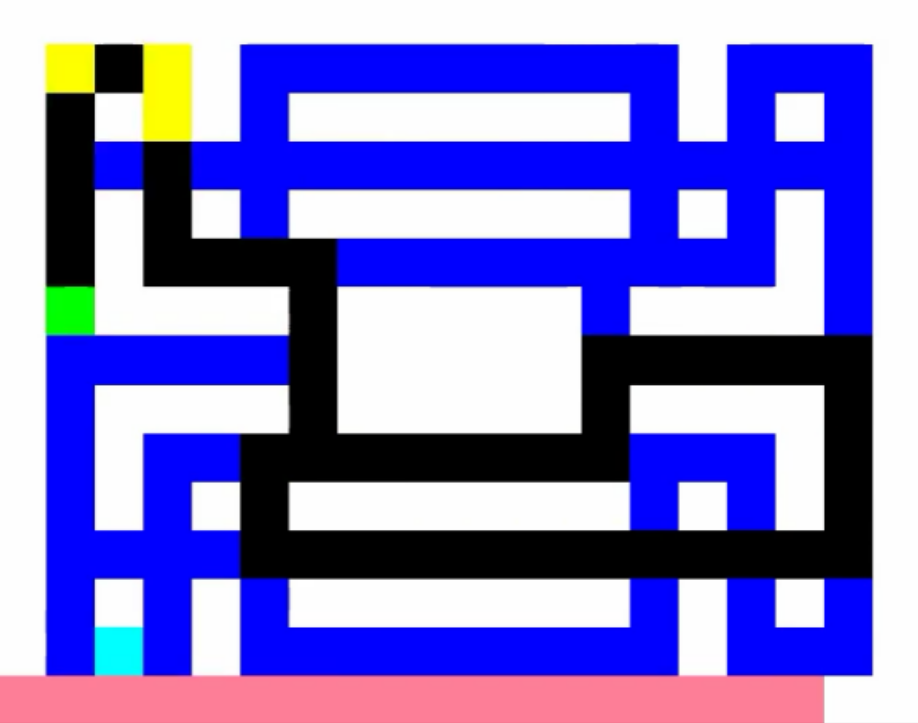
\includegraphics[width=0.5\columnwidth]{./Images/mini_pacman.png}
  \caption{Mini Pacman} 
  \label{fig:environment_model_architecture} 
\end{figure} 


I2A Model Based Path expensive to train
• Uses 15 x 19 Grid World version of Pacman
• Makes vision problem easier but preserves the reinforcement
learning problem
•
MiniPacman can be played in different modes



Hunt Rewards:\\

\begin{center}
	\begin{tabular}{ p{4cm}  r }
 	At each step & 0 \\
  	Eating food & 0 \\
	Eating power pill & 1\\
	Eating ghost & 10\\
	Killed by ghost & -20\\
	\end{tabular}
\end{center}